\documentclass{article}

\usepackage{graphicx}
\usepackage{tikz}
\usepackage{tikzsymbols}
\usetikzlibrary{calc,patterns,shapes.geometric}
\pagestyle{empty}
\usepackage[margin=0pt]{geometry}
\geometry{papersize={14in,12in}}

\def\centerarc[#1](#2)(#3:#4:#5){\draw[#1] ($(#2)+({#5*cos(#3)},{#5*sin(#3)})$) arc (#3:#4:#5);}

\begin{document}
	\begin{figure}
		\centering
		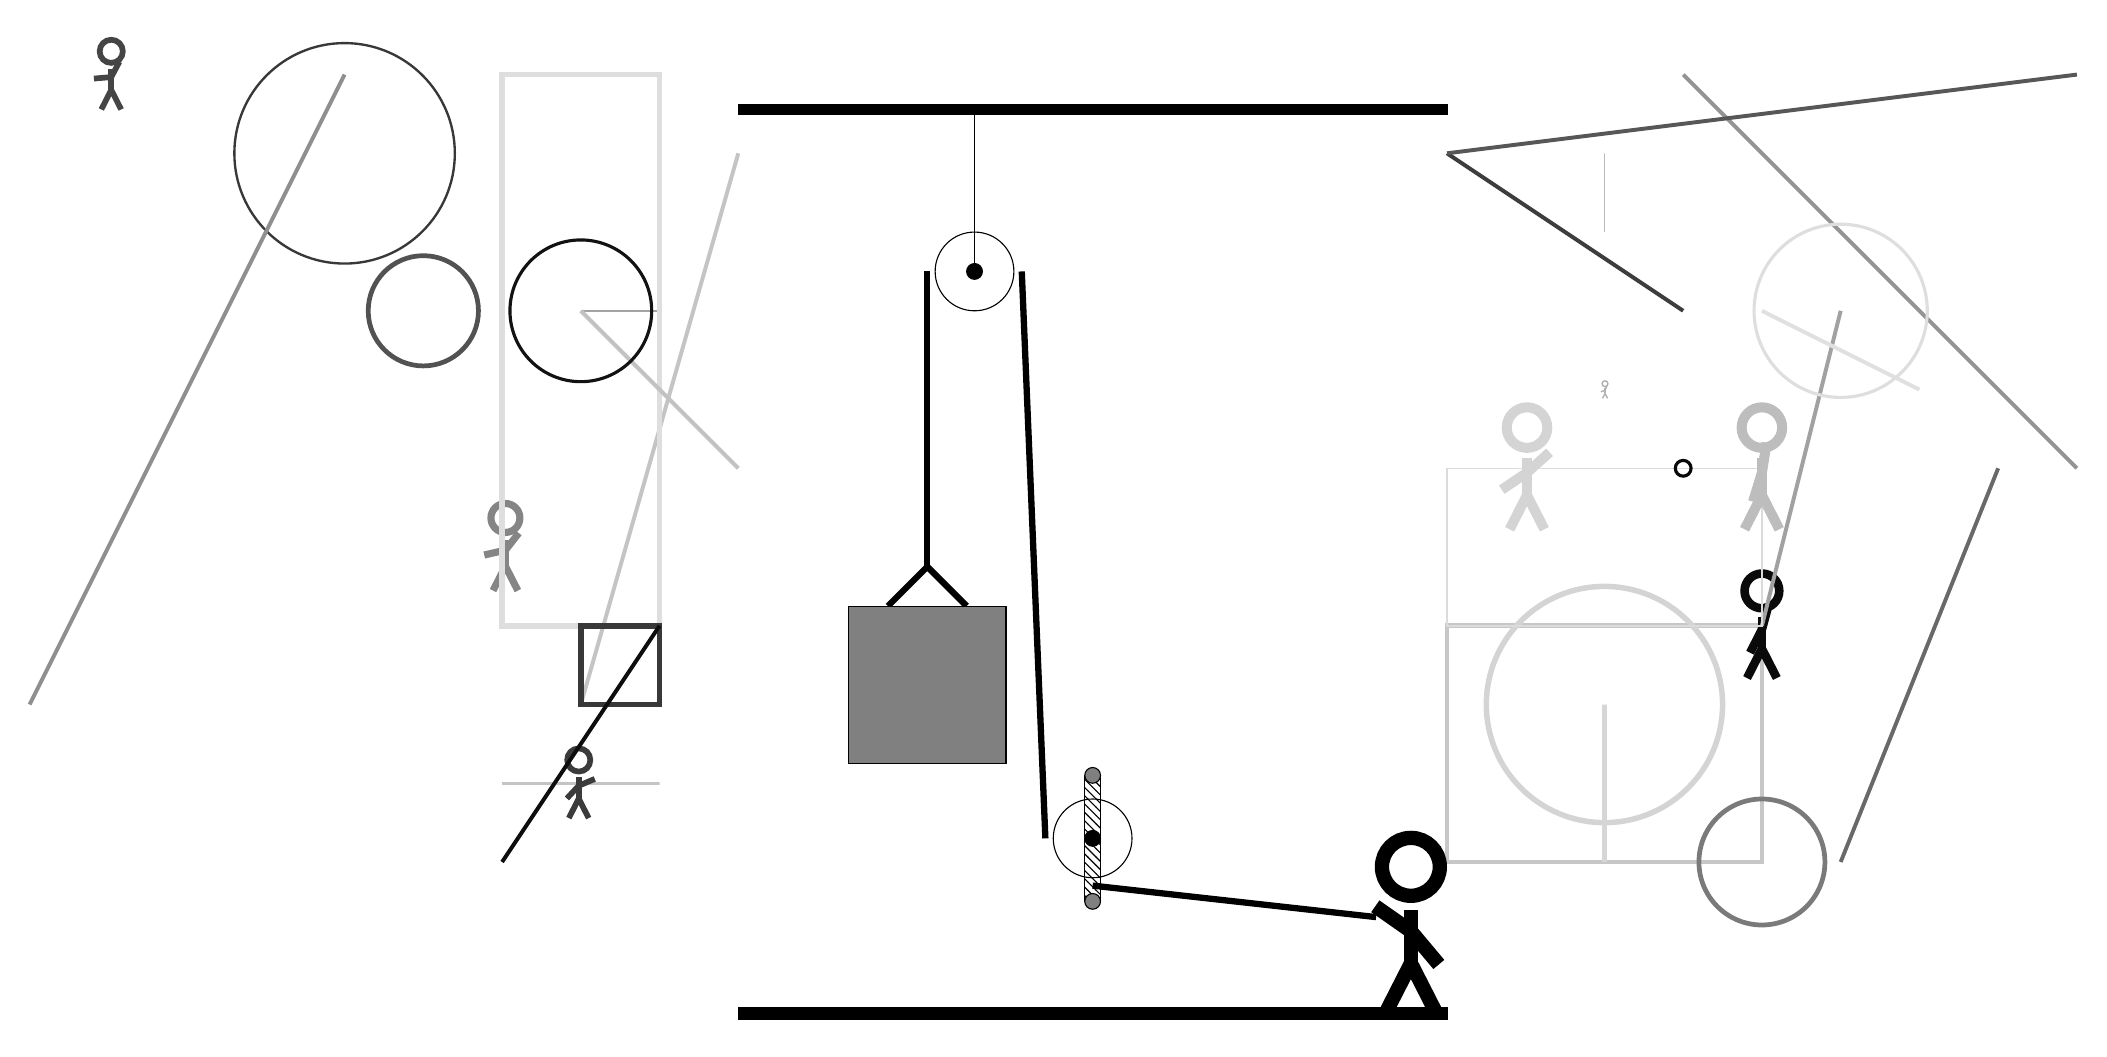
\begin{tikzpicture}
			%%%%% START %%%%%
			
			\draw[fill=black] (-2, 11.5) rectangle (7, 11.625);
			
			\node[line width=0.3mm, color=black!48] at (-5, 6) {\Strichmaxerl[5][13][52]};
			
			\node[line width=0.4mm, color=black!73] at (-10, 12) {\Strichmaxerl[4][5][62]};
			\draw[line width=0.5mm, color=black!42](10, 12) -- (15, 7);
			\draw [line width=0.3mm, color=black!78](-7, 11) circle (1.4);
			\draw[line width=0.6mm, color=black!22] (7, 5) rectangle (11, 2);
			
			\draw[line width=0.5mm, color=black!76](10, 9) -- (7, 11);
			\draw[line width=0.5mm, color=black!23](-2, 11) -- (-4, 4);
			\node[line width=0.7mm, color=black!31] at (9, 8) {\Strichmaxerl[1][22][66]};
			\draw[line width=0.2mm, color=black!27] (9, 10) rectangle (9, 11);
			\draw [line width=0.7mm, color=black!17](9, 4) circle (1.5);
			\draw[line width=0.4mm, color=black!23] (-3, 3) rectangle (-5, 3);
			
			\draw[line width=0.5mm, color=black!44](-7, 12) -- (-11, 4);
			\node[line width=0.4mm, color=black!77] at (-4, 3) {\Strichmaxerl[4][47][23]};
			
			\node[line width=0.5mm, color=black!96] at (11, 5) {\Strichmaxerl[6][63][75]};
			\draw[line width=0.5mm, color=black!37](12, 9) -- (11, 5);
			\draw[line width=0.2mm, color=black!36] (-4, 9) rectangle (-3, 9);
			
			\draw[line width=0.7mm, color=black!13] (-3, 12) rectangle (-5, 5);
			\draw[line width=0.5mm, color=black!59](12, 2) -- (14, 7);
			\draw[line width=0.5mm, color=black!24](-4, 9) -- (-2, 7);
			\draw[line width=0.2mm, color=black!14] (7, 5) rectangle (11, 7);
			\draw[line width=0.5mm, color=black!66](7, 11) -- (15, 12);
			
			\draw[line width=0.7mm, color=black!16] (9, 2) rectangle (9, 4);
			
			\draw [line width=0.4mm, color=black!13](12, 9) circle (1.1);
			\draw[line width=0.7mm, color=black!78] (-3, 4) rectangle (-4, 5);
			\node[line width=0.3mm, color=black!26] at (11, 7) {\Strichmaxerl[7][73][81]};
			
			\draw [line width=0.4mm, color=black!93](-4, 9) circle (0.9);
			\draw [line width=0.6mm, color=black!52](11, 2) circle (0.8);
			\draw[line width=0.5mm, color=black!12](11, 9) -- (13, 8);
			\node[line width=0.7mm, color=black!17] at (8, 7) {\Strichmaxerl[7][34][42]};
			\draw [line width=0.4mm, color=black!97](10, 7) circle (0.1);
			\draw[line width=0.5mm, color=black!95](-3, 5) -- (-5, 2);
			
			\draw [line width=0.6mm, color=black!68](-6, 9) circle (0.7);
			
			\draw (1, 9.5) circle (0.5);
			\draw[fill=black] (1, 9.5) circle (0.1);
			\draw (1, 11.5) -- (1, 9.5);
			
			\draw[fill=white](2.5, 2.3) circle (0.5);
			\draw[fill=black] (2.5, 2.3) circle (0.1);
			\draw[pattern=north west lines, pattern color=black] (2.4, 3.1) rectangle (2.6, 1.5);
			\draw[fill=black!50] (2.5, 3.1) circle (0.1);
			\draw[fill=black!50] (2.5, 1.5) circle (0.1);
			
			\draw[line width=0.8mm] (-0.1, 5.25) -- (0.4, 5.75) -- (0.9, 5.25);
			\draw[fill=black!50] (-0.6, 5.25) rectangle (1.4, 3.25);
			
			\draw[line width=0.8mm] (0.4, 9.5) -- (0.4, 5.75);
			\centerarc[line width=0.8mm](1, 9.5)(0:180:0.6);
			\draw[line width=0.8mm](1.6, 9.5) -- (1.9, 2.3);
			\centerarc[line width=0.8mm](2.5, 2.3)(180:270:0.6);
			\draw[line width=0.8mm](2.5, 1.7) -- (6.1, 1.3);
			
			\node at (6.5, 1.2) {\Strichmaxerl[10][-35][-50]};
			
			\draw[fill=black] (-2, 0) rectangle (7, 0.15);
			
			%%%%% END %%%%%
		\end{tikzpicture}
	\end{figure}	
\end{document}